\documentclass{article}
\usepackage[top=1in, bottom=1in, left=1.25in, right=1.25in]{geometry}
\usepackage{amsmath,amssymb}
\usepackage{xcolor}
\usepackage{graphicx}
\setlength{\parindent}{0pt}
\usepackage[utf8]{inputenc}
 
\usepackage{listings}
\usepackage{color}
 
\definecolor{codegreen}{rgb}{0,0.6,0}
\definecolor{codegray}{rgb}{0.5,0.5,0.5}
\definecolor{codepurple}{rgb}{0.58,0,0.82}
\definecolor{backcolour}{rgb}{0.95,0.95,0.92}
 
\lstdefinestyle{mystyle}{
    backgroundcolor=\color{backcolour},   
    commentstyle=\color{codegreen},
    keywordstyle=\color{magenta},
    numberstyle=\tiny\color{codegray},
    stringstyle=\color{codepurple},
    basicstyle=\footnotesize,
    breakatwhitespace=false,         
    breaklines=true,                 
    captionpos=b,                    
    keepspaces=true,                 
    numbers=left,                    
    numbersep=5pt,                  
    showspaces=false,                
    showstringspaces=false,
    showtabs=false,                  
    tabsize=2
}
 
\lstset{style=mystyle}

\title{ Bios/CS 534 Project 2}
\author{Chenxi Cai}
\begin{document}
\lstset{numbers=left, numberstyle=\small, keywordstyle=\color{blue!70}, commentstyle=\color{red!50!green!50!blue!50}, frame=shadowbox, rulesepcolor=\color{red!20!green!20!blue!20},escapeinside=``, xleftmargin=2em,xrightmargin=2em, aboveskip=1em}
\maketitle
\section{Problem 1}
With perceptron function, the error rate is
 			\begin{equation}
				0.033333  
				\end{equation} 

\textbf{Python codes of problem 1:}
\lstinputlisting[language=Python]{Proj2.1.py}

\section{Problem 2}
 With a function of Adaboost, the error rate is shown in Table below
 \begin{center}
\label{Adaboost}
\begin{tabular}{  l | c | c | c | r }

\hline
Iteration & 3 & 5 & 10 & 20 \\
\hline
Error rate & 0.167 & 0.167 & 0.133 & 0.133 \\
\hline
 \end{tabular}
\end{center}
Plot of Error rate vs iteration is shown as Fig.~\ref{Adaboost}
\begin{figure}[h]
    		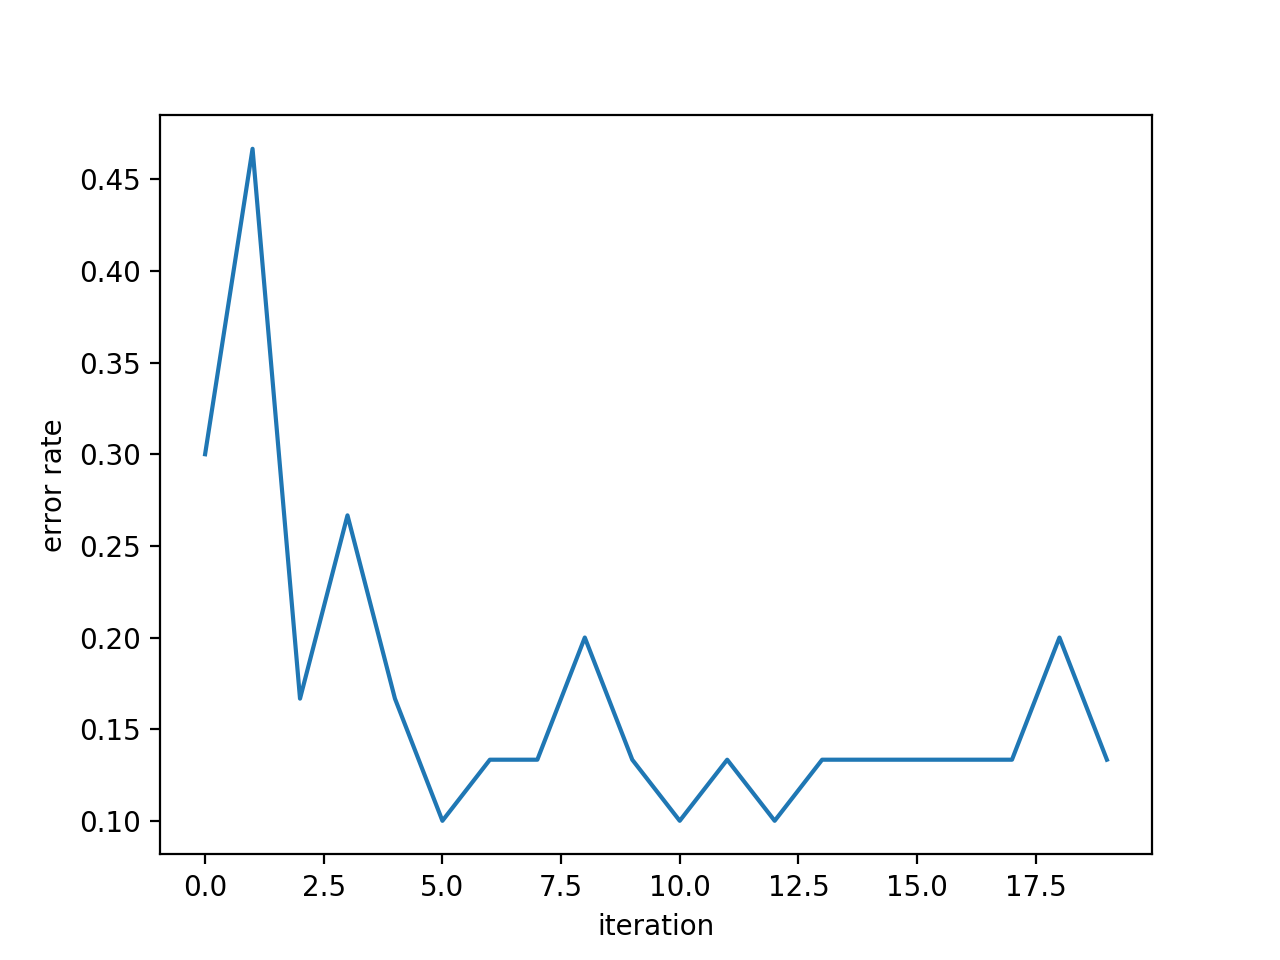
\includegraphics[width=5 in]{Adaboost.png}
		\centering
		\caption{Plots of Adaboost error rate}
		\label{Adaboost}
    		\end{figure}

\newpage
\textbf{Python codes of problem 2:}
\lstinputlisting[language=Python]{Proj2.2.py}

 
 \section{Problem 3}
 By using SVM in sklearn, the best parameter and error rate of three kernel methods are shown in Table  below
 
 \begin{center}
\label{SVM}
\begin{tabular}{  l | c |  c |  r }
\hline
     & Radical kernel  & Sigmoid kernel & Polynomial kernel  \\
\hline
Best parameter (gamma/degree)  & 0.02  & 0.06 & 2  \\
\hline
Error rate & 0.443 & 0.493 & 0.426 \\
\hline
 \end{tabular}
\end{center}
Plots of Scores vs gamma or degree of three kernels are shown as Fig.~\ref{radical},~\ref{sigmoid},~\ref{poly}
 
\begin{figure}[!hbp]
    		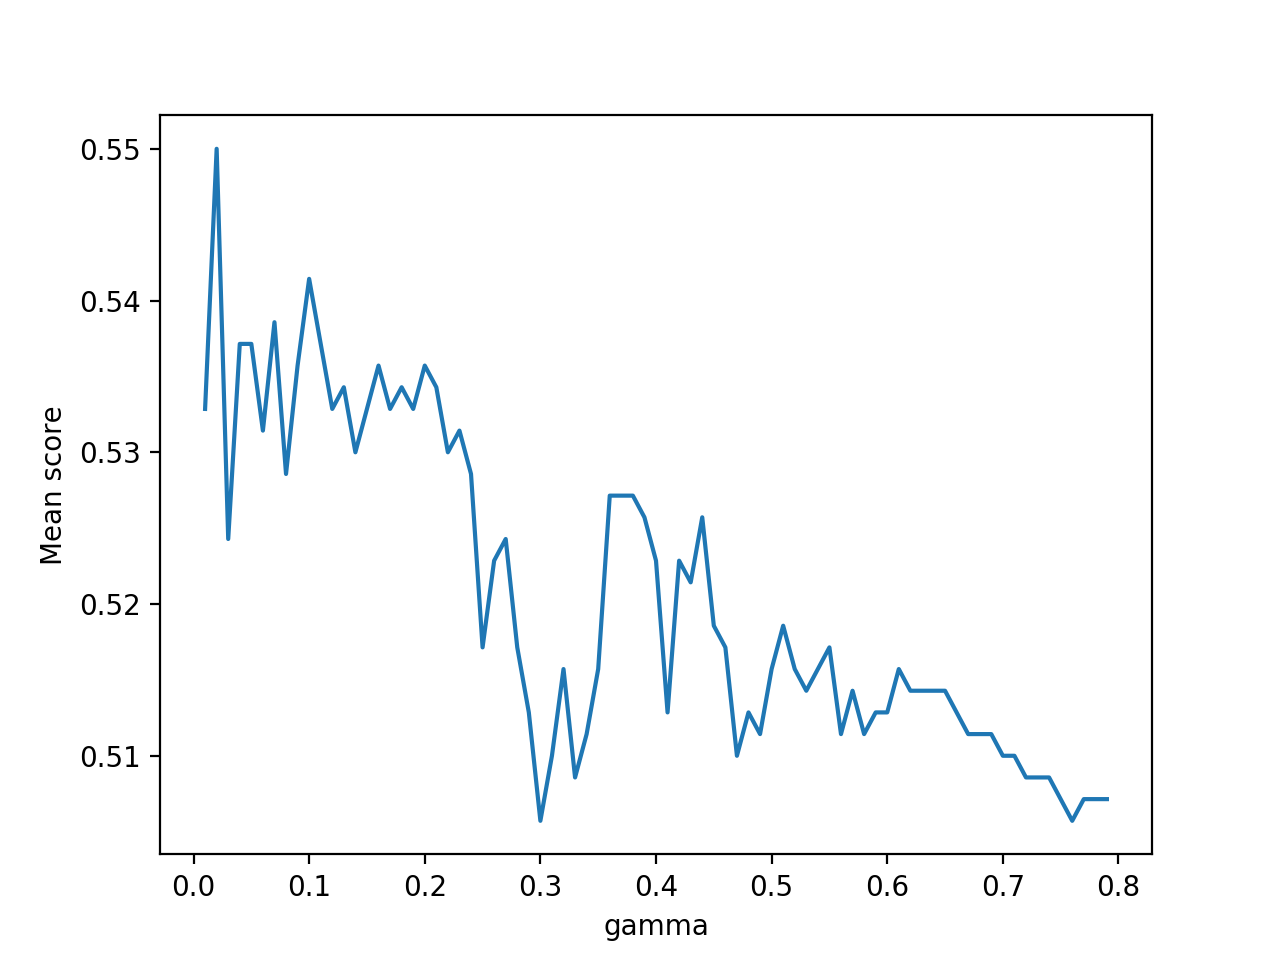
\includegraphics[width=5 in]{radical.png}
		\centering
		\caption{Plots of radical kernel}
		\label{radical}
    		\end{figure}
				\begin{figure}[!hbp]
    		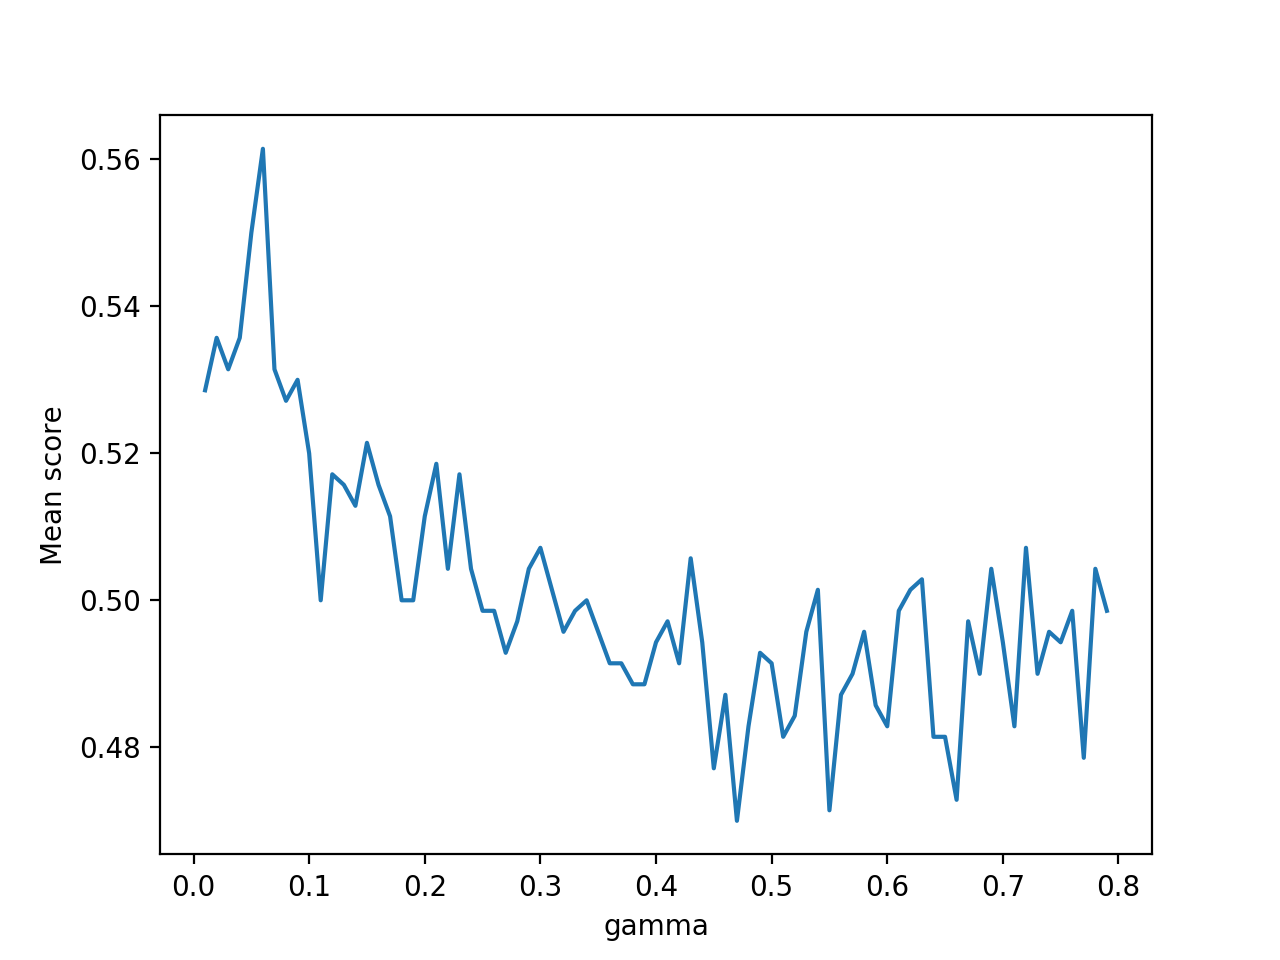
\includegraphics[width=5 in]{sigmoid.png}
		\centering
		\caption{Plots of sigmoid kernel}
		\label{sigmoid}
    		\end{figure}

				\begin{figure}[h]
    		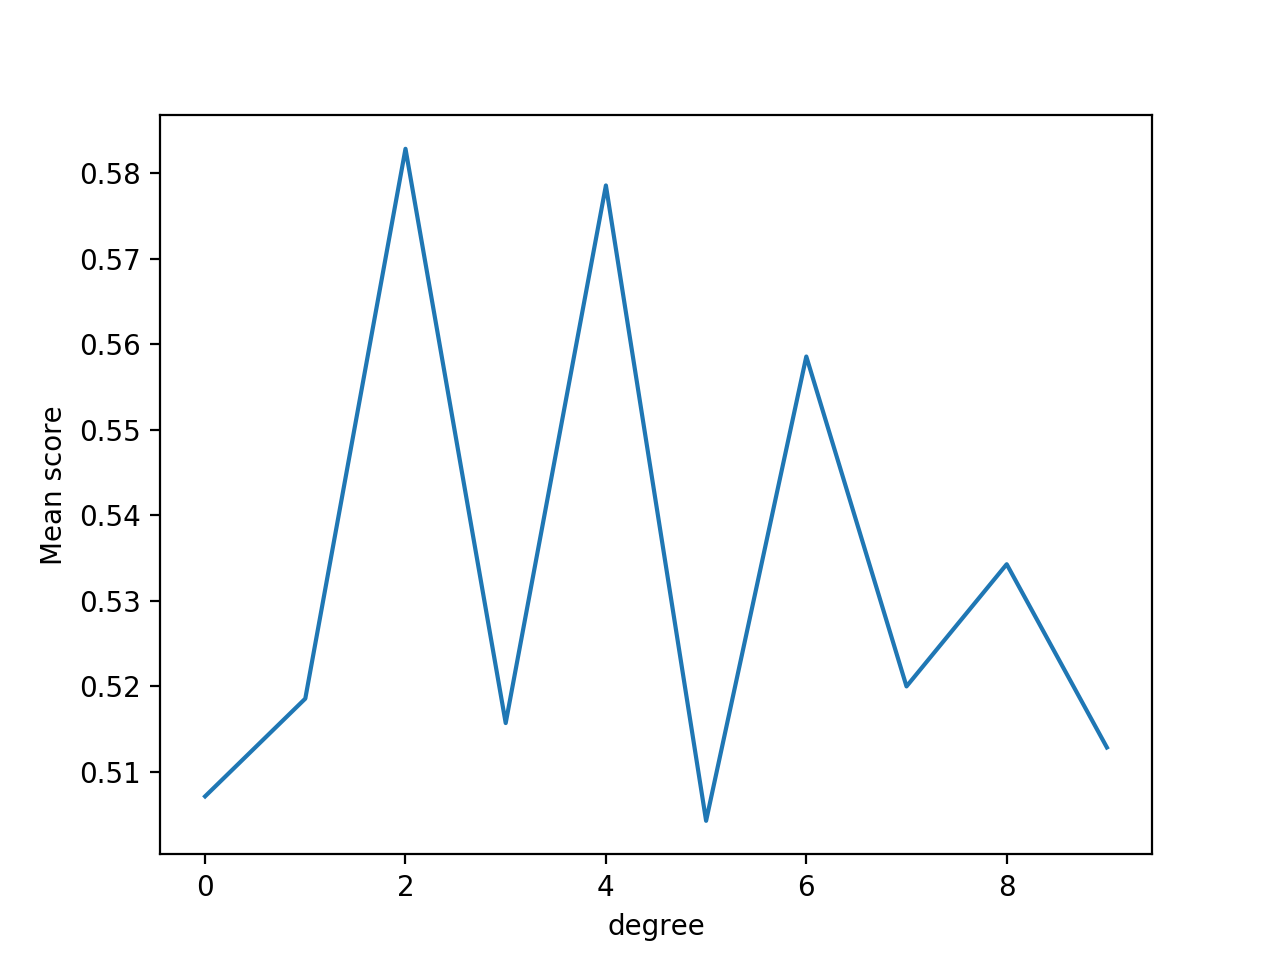
\includegraphics[width=5 in]{poly.png}
		\centering
		\caption{Plots of polynomial kernel}
		\label{poly}
    		\end{figure}

\newpage
\textbf{Python codes of problem 3:}
\lstinputlisting[language=Python]{Proj2.3.py}
				
\section{Problem 4}
The plot of OOB error rate and number of trees are shown in Fig.~\ref{forest}, 
\begin{figure}[!hbp]
    		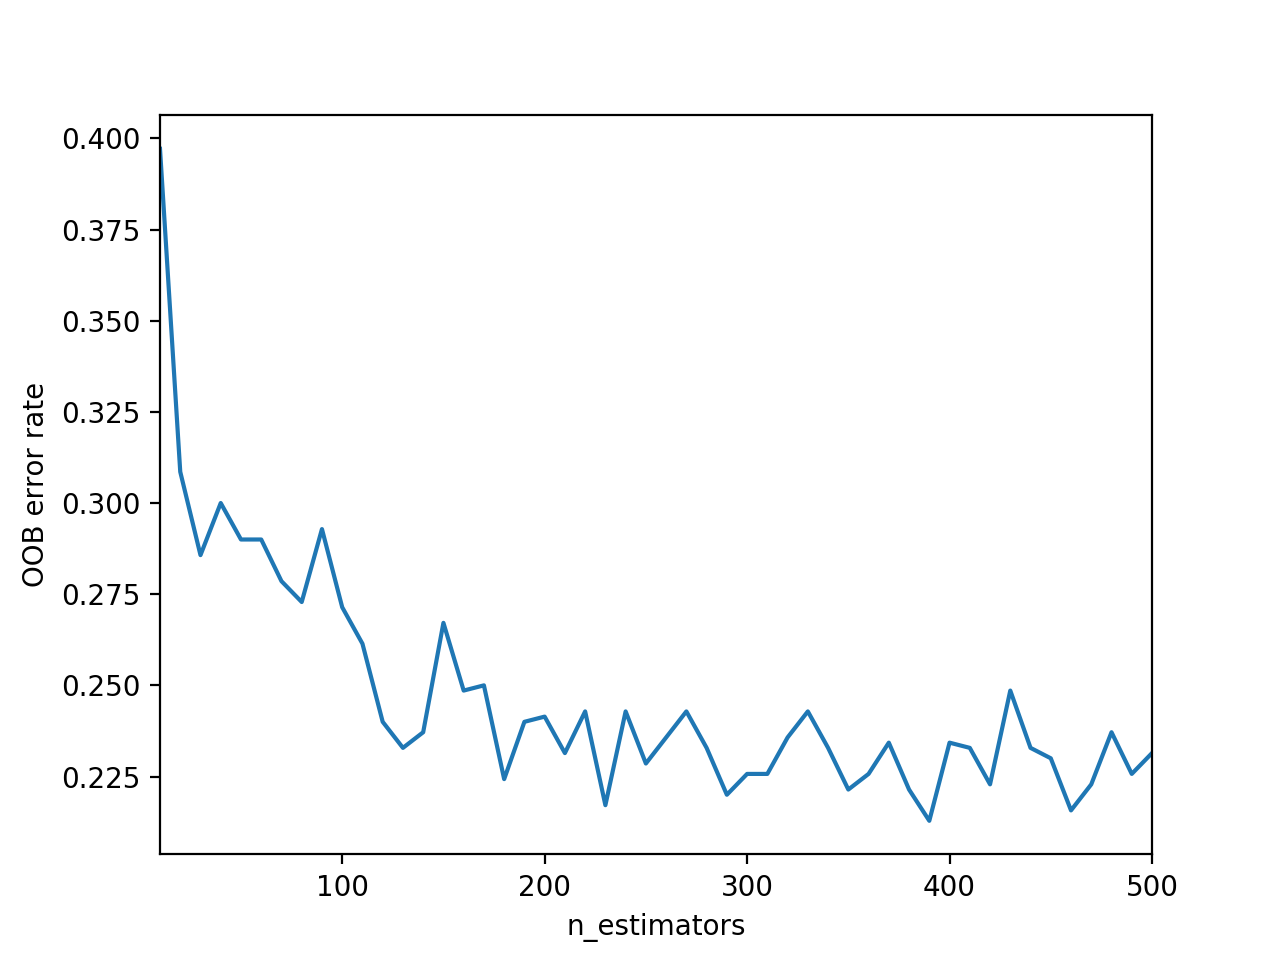
\includegraphics[width=5 in]{Forest.png}
		\centering
		\caption{plots of OOB error rate vs number of trees}
		\label{forest}
    		\end{figure}

The selected number of trees is 210, and the error rate is 

	\begin{equation}
				0.223333
				\end{equation}

The feature ranking is:
\begin{center}
\begin{tabular}{ l | c | r  }
\hline
rank & index of variables & importances \\
\hline
 1 & 4 &  (0.129395)\\
2 & 9 & (0.119601) \\
3 & 14 & (0.101843) \\
4 & 0 & (0.041882) \\
5 & 10 & (0.041192) \\
6 & 2 & (0.041054) \\
7 & 12 & (0.039885) \\
8 & 1 & (0.039104) \\ 
9 & 16 & (0.038682) \\
10 & 3 & (0.038664) \\ 
11 & 11 & (0.038254) \\
12 & 7 & (0.038123) \\
13 & 5 & (0.037836) \\
14 & 19 & (0.037576) \\
15 & 18 & (0.037312) \\
16 & 8 & (0.036664) \\
17 & 6 & (0.036404) \\
18 &13 &(0.036342) \\
19 & 15 & (0.035886) \\
20 & 17 & (0.034302) \\
\end{tabular}
\end{center}

\textbf{Python codes of problem 4:}
\lstinputlisting[language=Python]{Proj2.4.py}

\section{Problem 5}
By running gradient boosting with deviance loss on the training data, the error rate is
 			\begin{equation}
				0.193333
				\end{equation} 

The feature ranking is:
\begin{center}
\begin{tabular}{ l | c | r  }
\hline
rank & index of variables & importances \\
\hline
1 & 9 & (0.254537) \\
2. & 4 & (0.241189) \\
3 &14 & (0.215034) \\
4 & 1 & (0.034982) \\
5 & 10 & (0.031280) \\
6 & 3 & (0.023650) \\
7 & 7 & (0.023579) \\
8 & 6 & (0.020974) \\
9 & 2 & (0.020797) \\ 
10 & 18 & (0.020200) \\
11& 5 & (0.017700) \\
12 & 8 & (0.015834) \\
13 & 0 & (0.015096) \\
14 & 17 & (0.012983) \\ 
15 & 13 & (0.011701) \\
16& 11 & (0.010080) \\ 
17 & 19 & (0.008941) \\
18 & 16 & (0.008900) \\
19 & 15 & (0.007335) \\
20 & 12 & (0.005209) \\
\end{tabular}
\end{center}

\textbf{Python codes of problem 5:}
\lstinputlisting[language=Python]{Proj2.5.py}

\section{Problem 6}
With MARS, the error rate is
 			\begin{equation}
				0.24333
				\end{equation} 

\textbf{Python codes of problem 6:}
\lstinputlisting[language=Python]{Proj2.6.py}



\end{document}